\documentclass[11pt]{article}
\usepackage{graphicx}
\usepackage{fullpage}

\title{CS63 Spring 2026\\Lab 8: Convolutional Neural Networks}
\author{Jaden Jones and Reishiro Kawakami}
\date{}

\begin{document}

% Look in /home/meeden/public/latex-example for an example of how
% to inclue figures and create tables in your latex document.

\maketitle

\section{Data Set}
The dataset contains 70,000 clothes images of size 28 x 28 pixes, with each image labeled with a target label. The possible target labels are as follows: 

\begin{itemize}
  \item 0 = t-shirt
  \item 1 = trouser
  \item 2 = pullover
  \item 3 = dress
  \item 4 = coat
  \item 5 = sandal
  \item 6 = shirt
  \item 7 = sneaker
  \item 8 = bag
  \item 9 = ankle boot
\end{itemize}


\section{Network}

% TODO Summarize the best performing network architecture you created.
% Remember that we are defining best in terms of validation results.

The best performing network we created was a result of pooling the "shirt" and "t-shirt" categories into, 
which seemed vague from a human perspective, into the more general "pullover" category. This was partly motivated 
by the data in the confusion matrix, which indicated that these two categories were getting 
easily confused for each other. Additional accuracy was gained by increasing the number of training 
epochs from 5 to 15. 

% TODO Include a screen shot of the summary of the network.
\begin{figure}[h]
    \centering
    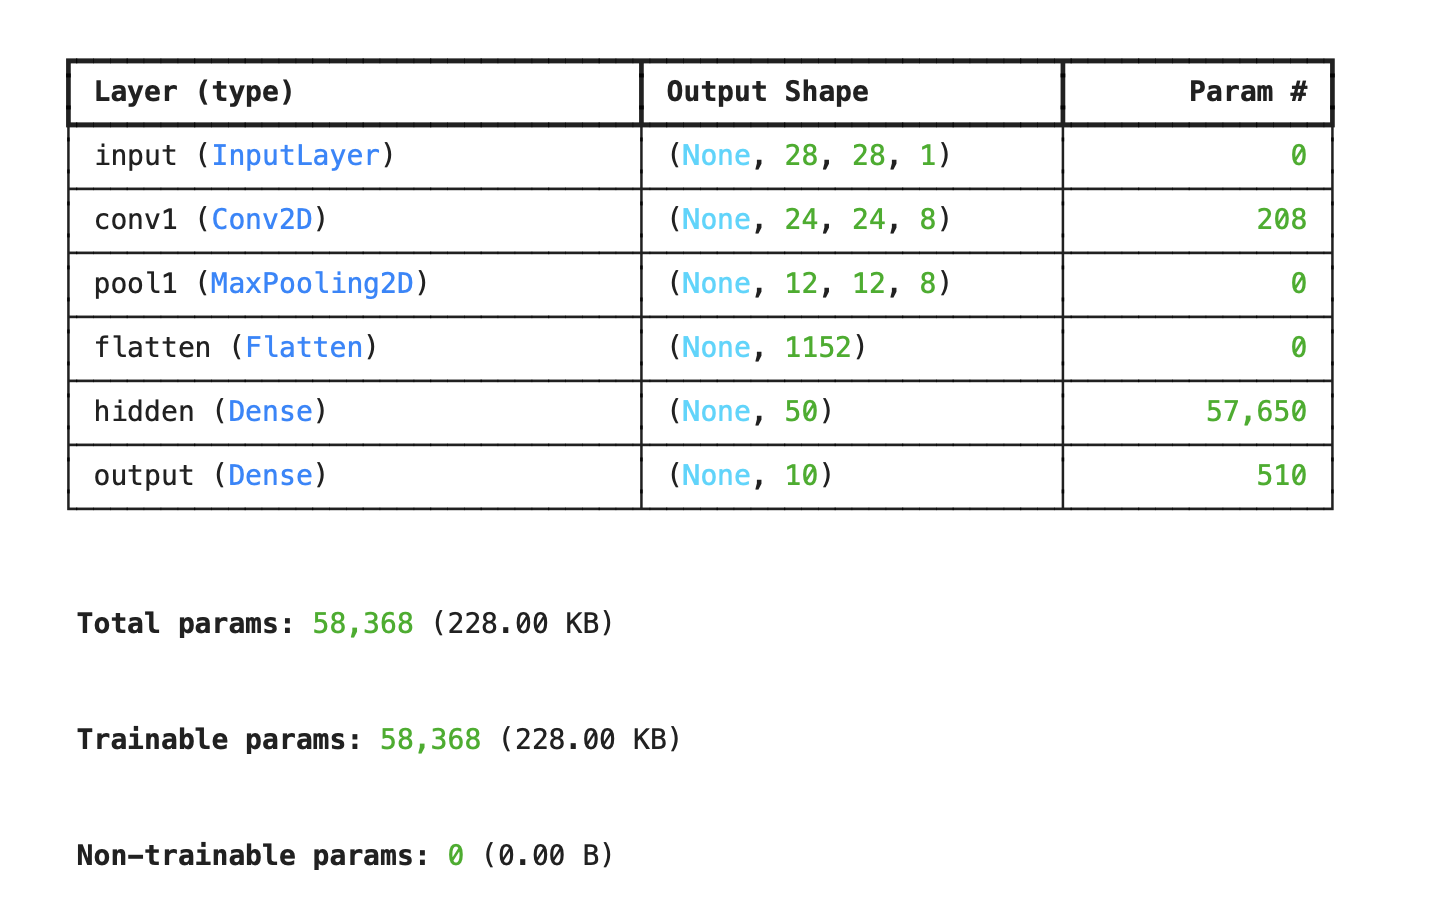
\includegraphics[width=1\textwidth]{SeqNetSummary.png}
    \caption{The summary of the network}
    \label{fig:my_label}
\end{figure}
% TODO If you have any insight into why it performed well, explain. 


\section{Training}

% TODO Run your network from scratch at least 5 times.

% TODO Include a table showing the validation results of each of the runs
% as well as the average performance over all runs.

\begin{tabular}{|l|c|r|}
  \hline
  Run & Accuracy & Val Accutacy  \\ \hline
  1 & 0.932 & 0.922 \\
  2 & 0.935 & 0.923 \\
  3 & 0.936 & 0.927 \\
  4 & 0.935 & 0.927 \\
  5 & 0.936 & 0.917 \\ \hline
  Average & 0.935 & 0.923 \\ \hline
\end{tabular}

% TODO Include a screen shot of a typical learning graphs from these runs.
\begin{figure}[h]
    \centering
    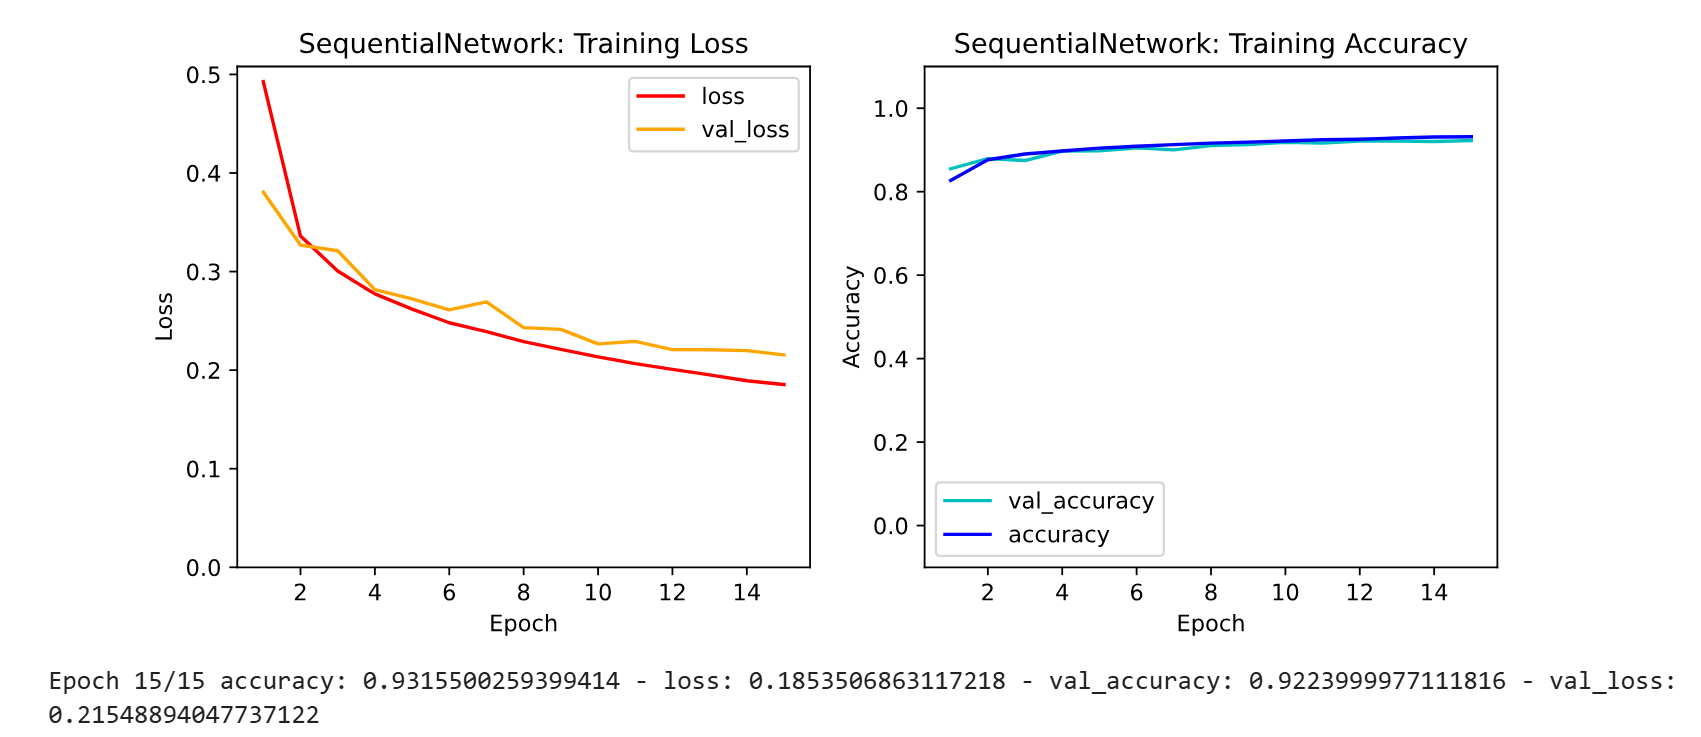
\includegraphics[width=1\textwidth]{run1.png}
    \caption{A typical learning graphs}
    \label{fig:my_label}
\end{figure}

\section{Evaluation}

\begin{figure}[h]
    \centering
    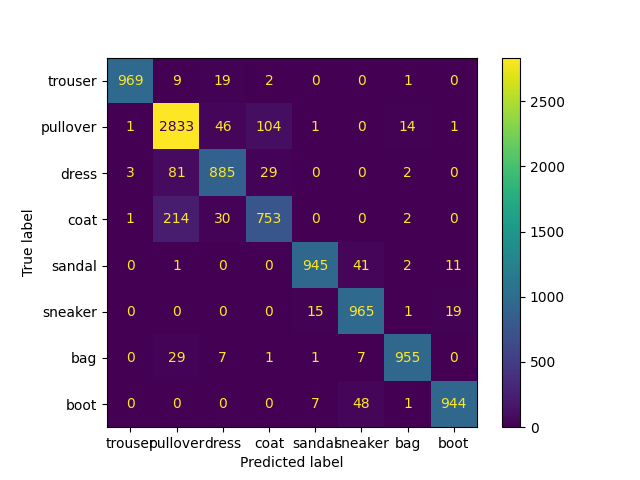
\includegraphics[width=1\textwidth]{cm.png}
    \caption{The confusion matrix}
    \label{fig:my_label}
\end{figure}

The network performed well on trousers and sneakers. This is probably because these clothes have distinct feature maps. The trousers have the edges for legs, which is a distinct feature of trousers in the dataset, and the model was focused on the feature (see figure 4). It may have been more difficult if the dataset included shorts. The sneakers had high accuracy probably because of the relatively distinctions between boots (figure 5), sneakers (figure 6), and sandals (figure 7). The feature maps showed that the model was focusing on the upper edge of the shoes, which was consistenyl a steep curve for boots, a little blurry for sandals, and rather flat for sneakers. 

\begin{figure}[h]
    \centering
    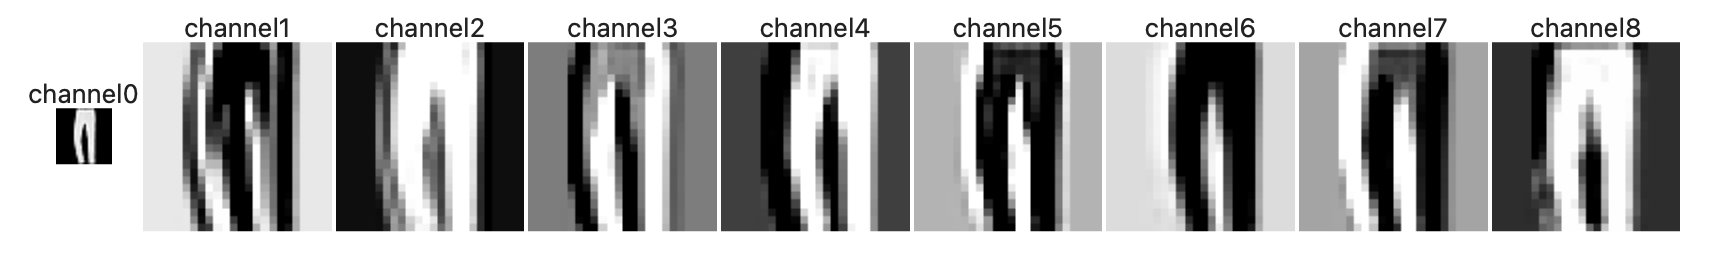
\includegraphics[width=1\textwidth]{trouser_featuremap.png}
    \caption{The feature map of a trouser}
    \label{fig:my_label}
\end{figure}
\begin{figure}[h]
    \centering
    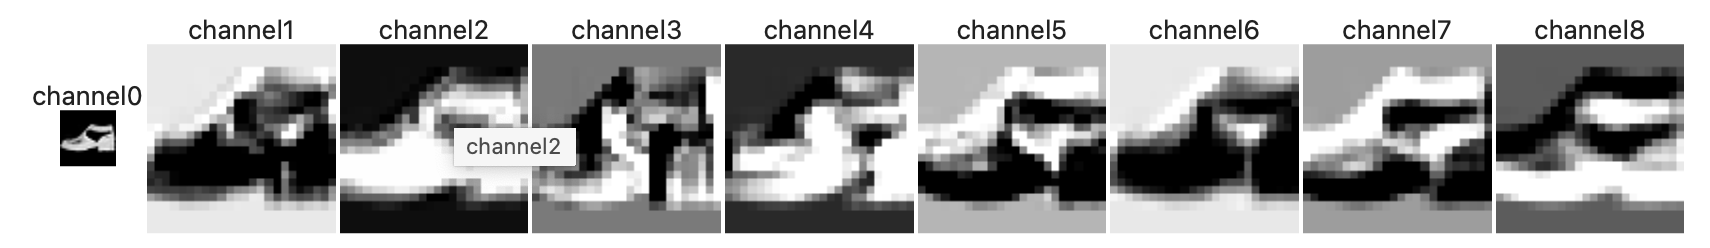
\includegraphics[width=1\textwidth]{boot_featuremap.png}
    \caption{The feature map of a boot}
    \label{fig:my_label}
\end{figure}
\begin{figure}[h]
    \centering
    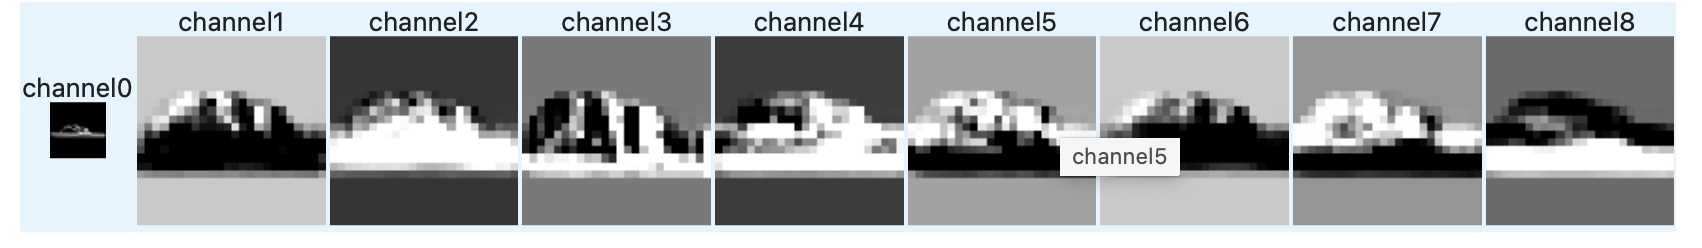
\includegraphics[width=1\textwidth]{sandals_featuremap.png}
    \caption{The feature map of a sandal}
    \label{fig:my_label}
\end{figure}
\begin{figure}[h]
    \centering
    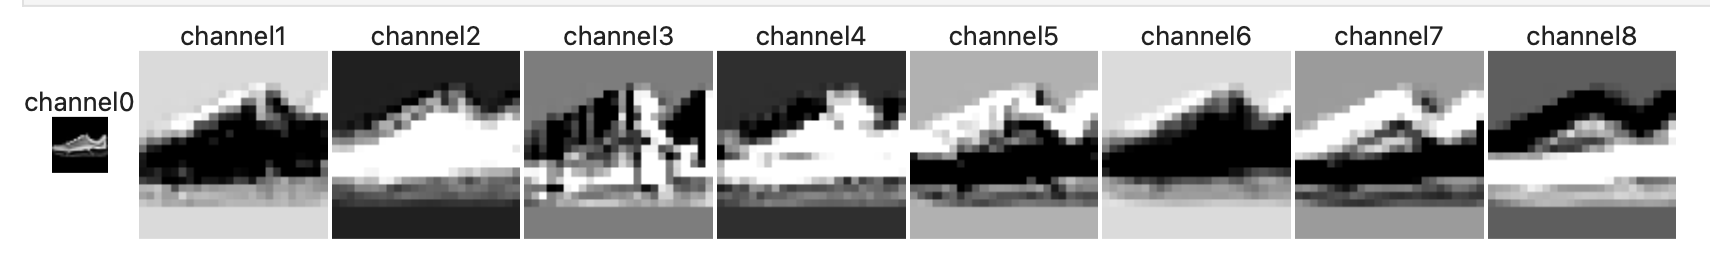
\includegraphics[width=1\textwidth]{sneaker_featuremap.png}
    \caption{The feature map of a sneaker}
    \label{fig:my_label}
\end{figure}


On the other hand, the network performed poorly for coat, pullover, and dress in terms of the raw counts. This seems relatively reasonable considering their similarities -- we felt that even humans would struggle to distinguish between these three for some of the images. When we look at the feature maps, we can tell that the model is focused on the arms (and a little bit of the collars) when it comes to coat and pullover. However, arms are common features between coat and pullover. The feature map for dress also focuses on the edges around the torso of the dress, which looks the the arms of pullovers. Therefore, we think the model is focusing on the parts (i.e. arms) that don't really let the model to distinguish between these categories. 

\begin{figure}[h]
    \centering
    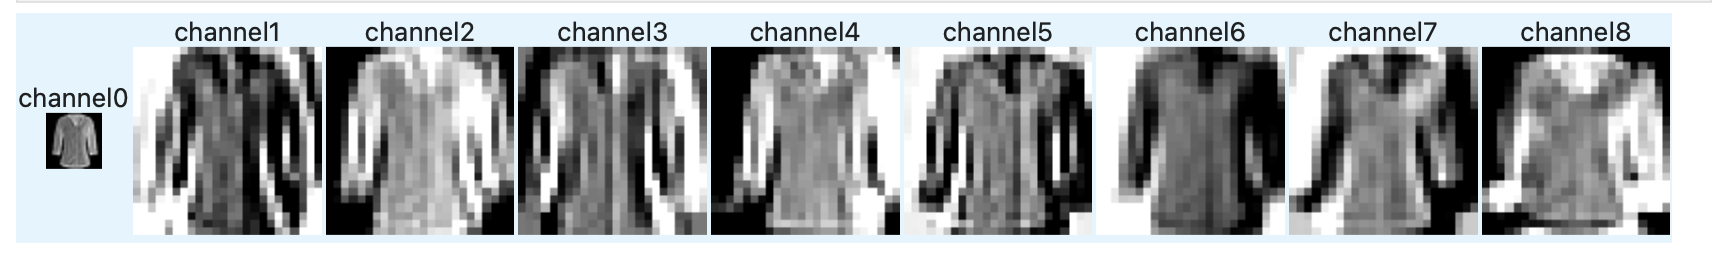
\includegraphics[width=1\textwidth]{pullover_featuremap.png}
    \caption{The feature map of a pullover}
    \label{fig:my_label}
\end{figure}

\begin{figure}[h]
    \centering
    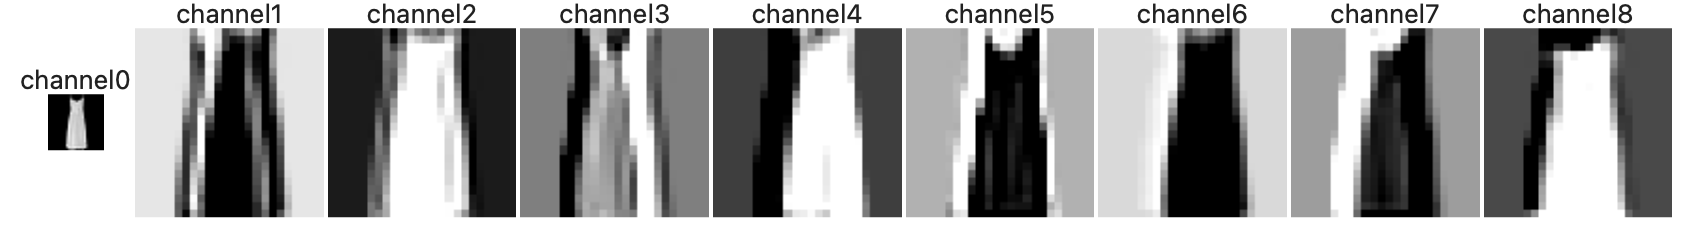
\includegraphics[width=1\textwidth]{dress_featuremap.png}
    \caption{The feature map of a dress}
    \label{fig:my_label}
\end{figure}

% TODO Explain what your network was good at and why.
% TODO Explain what your network was bad at and why.


% TODO Include screenshots of the feature maps of convolution and/or
% pooling layers to support your analysis. 


\end{document}
